% Licensed to the Apache Software Foundation (ASF) under one or more
% contributor license agreements. See the NOTICE file distributed with
% this work for additional information regarding copyright ownership.
% The ASF licenses this file to You under the Apache License, Version 2.0
% (the ``License''); you may not use this file except in compliance with
% the License. You may obtain a copy of the License at
%
% http://www.apache.org/licenses/LICENSE-2.0
%
% Unless required by applicable law or agreed to in writing, software
% distributed under the License is distributed on an ``AS IS'' BASIS,
% WITHOUT WARRANTIES OR CONDITIONS OF ANY KIND, either express or implied.
% See the License for the specific language governing permissions and
% limitations under the License.

\subsubsection{Configuring a Meridio Repository}

You must fill in the following extra fields if you choose to
configure a Meridio repository connection: 

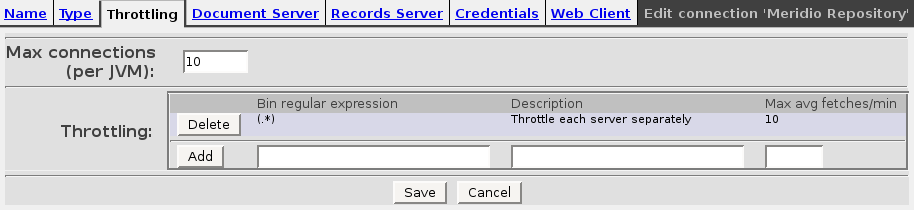
\includegraphics[width=300pt]{mer-edit-repository-tab3}


\begin{itemize}

\item \textbf{Max connections (per JVM):} Here you can set the maximum
number of connections to your repository.

The maximum number of connections per JVM is important for three
reasons.  First, the number of connections may impact the resources
available on your Meridio server. As in the case of the authority
connection, other demands on your Meridio server as well as the
maximum number of conections your server is configured to accept will
influence the number of connections you input here.

Second, the number of connections may impact the resources
available on the appliance. If the connector framework is slowing down
your appliance, lowering this number should help.

Third, only ten document streams can be processed by the appliance at
one time.  If you are also using other repository connectors or the
\command{ingest} command on the appliance, you should reduce this
number to prevent contention for the Ingestion interface. The
Meridio Connector will never overwhelm the interface on its own,
but when other applications are also using the ingestion interface, it
may be best to set the number of repository connections to five or
even fewer.

\item \textbf{Throttling:} Throttling allows you to limit the rate of
document ingestion based on document bin.

The maximum fetch rate allows you to set three things: Expression,
description, and fetches per minute. Each document is part of two
bins: one based on document service and one based on record
service. You can throttle documents from each service individually by
using the expression \texttt{(.*)}, or you can use a blank expression
to throttle all fetches for Meridio crawls together.

% This doesn't make sense to me. So you can only throttle "all fetches" 
% or "these two groups separately?" Why does "pick everything" mean
% "throttle separately?"

\end{itemize}

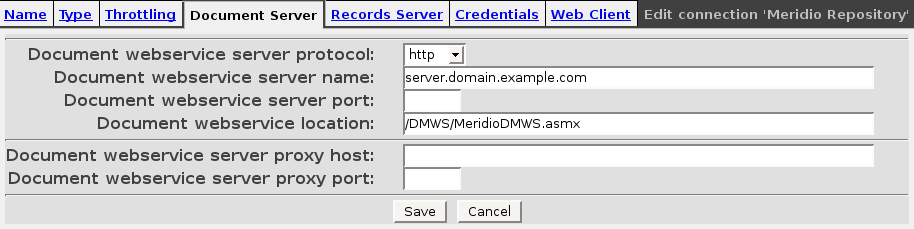
\includegraphics[width=300pt]{mer-edit-repository-tab4}


This tab specifies information about the Meridio document service that
you wish to crawl. You may need to ask your Meridio administrator for
this information. This should be the same information you provided
when creating the Meridio authority connection that you chose to use
with this repository connection.

\begin{itemize}

\item \textbf{Document webservice server protocol:} The appropriate protocol used by your Meridio document webservice.

\item \textbf{Document webservice server name:} The name of the server hosting your Meridio document webservice.

\item \textbf{Document webservice server port:} The port used to connect to the Meridio document webservice.

\item \textbf{Document webservice location:} The location of the Meridio document webservice on the server specified above. By default, the location of the service is given as \dirpath{/DMWS/MeridioDMWS.asmx}.

\item \textbf{Document webservice server proxy host:} If your MetaCarta appliance must connect to the server hosting the Meridio document webservice using a proxy, specify the name of the appropriate proxy host here.

\item \textbf{Document webservice server proxy port:} The port used to connect to the proxy host.

\end{itemize}

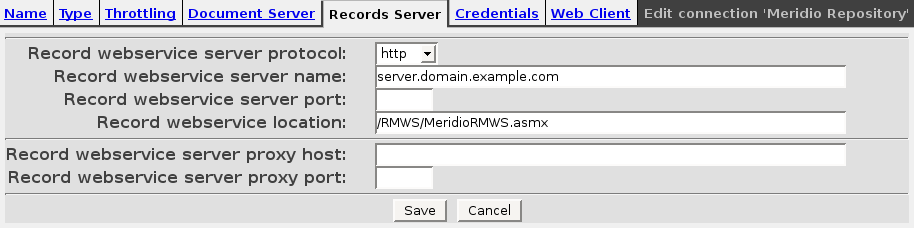
\includegraphics[width=300pt]{mer-edit-repository-tab5}

This tab specifies information about the Meridio record service
corresponding to the document service that you wish to crawl. You may
need to ask your Meridio administrator for this information. Some of
this information may be the same as from the previous tab, as a server
may host more than one Meridio service.  This should be the same
information you provided when creating the Meridio authority
connection that you chose to use with this repository connection.

\begin{itemize}

\item \textbf{Record webservice server protocol:} The appropriate protocol used by your Meridio record webservice.

\item \textbf{Record webservice server name:}  The name of the server hosting your Meridio record webservice.

\item \textbf{Record webservice server port:} The port used to connect to the Meridio record webservice.

\item \textbf{Record webservice location:} The location of the Meridio record webservice on the server specified above. By default, the location of the service is given as \dirpath{/RMWS/MeridioRMWS.asmx}

\item \textbf{Record webservice server proxy host:} If your MetaCarta appliance must connect to the server hosting the Meridio record webservice using a proxy, specify the name of the appropriate proxy host here.

\item \textbf{Record webservice server proxy port:} The port used to connect to the proxy host.

\end{itemize}


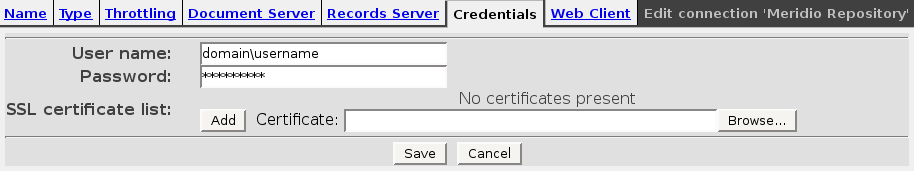
\includegraphics[width=300pt]{mer-edit-repository-tab6}


\begin{itemize}


\item \textbf{User name:} The Active Directory user name that the appliance should use when connecting to the Meridio services, in the form \texttt{domain$\backslash{}$username}. This should be an account created specifically for the appliance that you specified when creating the corresponding authority connection.

\item \textbf{Password:} The password for that account.

\item \textbf{SSL certificate list:}
You can upload SSL certificates to use with this connection here. If
you specified ``https'' as the server protocol above, you may need to
upload appropriate certificates or certificate authorities here. The
repository connection will need certificates similar to those used to
connect to your Meridio web service using an Internet browser.


If the certificate authority used to sign your server certificate is a
well-known authority, you will not need to upload a certificate
here. The appliance will automatically accept a certificate from the
server. If the server certificate is signed by an unknown authority,
you should upload the authority's certificate. In some cases, the
authority may be unavailable. In this case, you can upload the
server-side certificate itself. Server-side certificate changes may
require you to upload newer versions of this certificate if you use
this option.



\end{itemize}


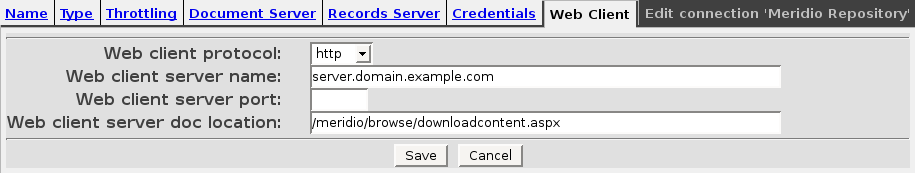
\includegraphics[width=300pt]{mer-edit-repository-tab7}

This tab specifies information about the web client service that can
be used to view the documents and records that are being processed by
the crawler. The information you provide here is used by the appliance
to generate retrieval URLs that are shown to appliance users. You may
need to ask your Meridio administrator for this information. Some of
this information may be the same as from previous tabs, as a server
may host more than one Meridio service.

\begin{itemize}

\item \textbf{Web client server protocol:}  The appropriate protocol used by your Meridio web client service.

\item \textbf{Web client server name:}  The name of the server hosting your Meridio web client service.

\item \textbf{Web client server port:}  The port used to connect to the Meridio web client service.

\item \textbf{Web client server doc location:}  The location of the Meridio web client service on the server specified above. By default, the location of the service is given as \dirpath{/meridio/browse/downloadcontent.aspx}.

\end{itemize}

After entering this information, you will be taken to the status page
for this repository connection:

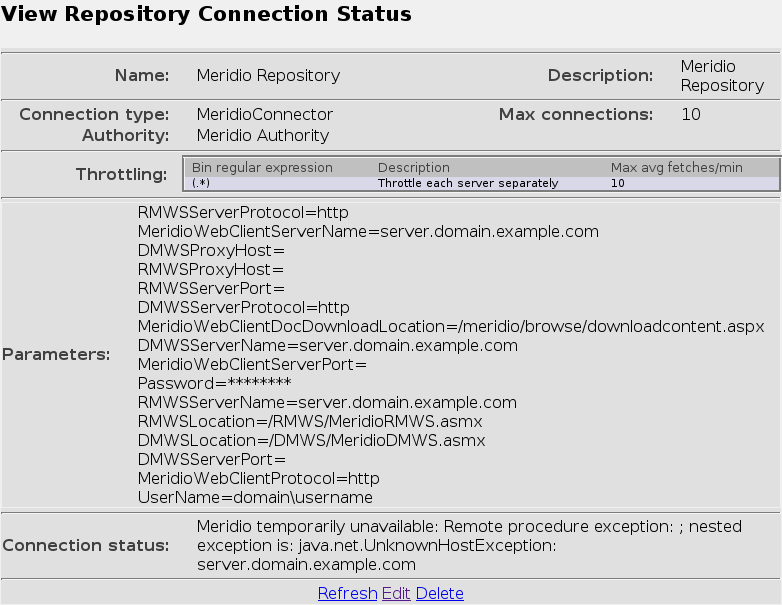
\includegraphics[width=300pt]{mer-view-repo-conn-status}

In this example (which does not contain accurate information for
any Meridio server), the Connection Status is ``Meridio temporarily
unavailable.''  If you see this message, your Meridio services may not be
responding, or you might have incorrectly entered one of the fields, and
should click ``Edit'' to fix the data. If you have entered everything as
you intended,  and the Meridio services are up, please inform your Meridio
administrator; you may not have been given the correct information.

